\chapter{Software Requirement Specification}
\\
{\normalsize {In the previous chapter, the literature survey is summarized. A software requirements specification is the basis for the entire project. It’s used to provide critical information to multiple teams - development, quality assurance, operations, and maintenance. Using the SRS helps to ensure requirements are fulfilled. And it can also help you make decisions about your product’s lifecycle for instance when to retire a feature. In this chapter, SRS is framed to identify requirements for the whole system.}}
\clearpage
\section{Introduction}
{\normalsize {Real Time Translation provides an intelligent, natural and convenient way of human-computer-interaction (HCI). Speech-to-Text and Text-to-Speech are two major applications for real time translation system. Real Time Translation aims to automatically translate from one language to another language.}}
\subsection{Project Scope}
{\normalsize{This project aims to help the people during meetings by helping them understand what the presenter is speaking in their native language}}
\subsection{Assumptions and Dependencies}
{\normalsize{\textbf{Assumptions:}}}
\begin{enumerate}
    \item The application is interfaced with high speed internet connectivity. 
    \item The system recovers automatically in case of any failure. 
\end{enumerate}
{\normalsize{\textbf{Dependencies:}}}
\begin{enumerate}
    \item Using API calls for calling the server
\end{enumerate}

\newpage
\section{Nonfunctional Requirements}
{\normalsize{The below point mention non-functional requirements to make the system more secure, faster and get best results from the system in terms of performance, reliability, security, manageability, etc.}}

\subsection{Performance Requirements}
{\normalsize{The latency for the retrieval of the working of system for speech to speech model must be less than 10 sec. The availability of the system should be as maximum as possible.}}


\subsection{Reliability Requirements}
{\normalsize{The network must stay reliable in case any of the system function fails. The normal execution of the system must not be affected by the system failure. The restoration procedure must be performed automatically. In case of failure of the system, the automatic restart procedure must be applied to provide full availability.}}

\subsection{Security Requirements}
{\normalsize{\textbf{API Calls:}}}
\\
{\normalsize{\textbf{Data Storage:}}}

\subsection{Software Quality Attribute}
\begin{enumerate}
    \item Efficiency: System fulfillment its purpose with utilization of all necessary resources.
    \item Portability: The ease with which a system can be adapted to run on computers. 
    \item Testability: Suitability for allowing to follow program execution. 
    \item Readability: Form of representation is understandable.
\end{enumerate}

\newpage
\section{System Requirements}
\subsection{Hardware Requirements}
{\normalsize{Following are hardware requirements for development of system: }}
\begin{itemize}
    \item Processors: Intel Atom R processor or Intel R CoreTM i3 processor and above. 
    \item Disk space (RAM): 4 GB 
    \item Hard Disk Space: 10 GB
\end{itemize}

\subsection{Software Requirements}
\begin{itemize}
    \item Operating systems: Windows 7 or later, macOS, and Linux 
    \item Compatible tools: Microsoft Visual Studio, PyCharm, C++ Editor    
    \item Python versions: 2.7.X, 3.6.X 
    \item Web Browser: - Google Chrome/Mozilla Firefox
\end{itemize}

\newpage
\section{Analysis Models: SDLC Model to be applied}
{\normalsize{\textbf{Iterative Model}}} 
{\normalsize{\par Implementation of SDLC that focuses on an initial, simplified implementation which then progressively gains more complexity and a broader feature set until the final system is complete.}}

\vspace*{0.2cm}
\begin{figure}[h]
  \begin{center}
  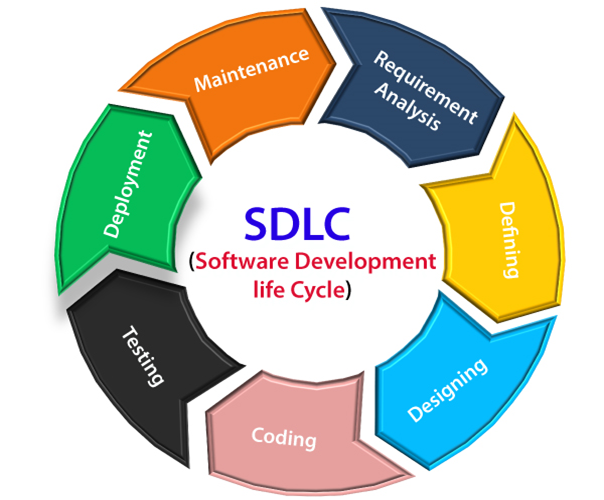
\includegraphics[height=80mm]{Images/Figures/software-engineering-software-development-life-cycle.jpeg}
  \caption{Iterative Model}
  \end{center}
\end{figure}

\vspace*{0.2cm}
\newpage
{\normalsize{The iterative model is used for building of our system because the modules are to be deployed independently which requires testing, validation, verification. Steps consist of: }}
\begin{enumerate} 
    \item Requirement Analysis
    \item Defining Requirements
    \item Designing
    \item Implementation 
    \item Testing
    \item Deployment
    \item Maintenance
\end{enumerate}

{\normalsize{The process of building the speech-to-speech translation model system consists of two steps: }}
\begin{enumerate}
    \item Building the speech-to-speech model system, independently testing the system.
    \item The system is tested to form the final system which is ready to be deployed.
    \item Both of the modules are integrated and tested to form the final system which is ready to be deployed.
\end{enumerate}